\documentclass{article}
\usepackage[utf8]{inputenc}
\usepackage{tabularx} % extra features for tabular environment
\usepackage{amsmath}  % improve math presentation
\usepackage{graphicx} % takes care of graphic including machinery
\usepackage{xspace}
\usepackage{tikz}
\usepackage{enumitem}
\usetikzlibrary{babel}
\usepackage[american]{circuitikz}
\usetikzlibrary{calc}
\usepackage{siunitx}
\usepackage{pgfplots}
\usepackage[skins,theorems]{tcolorbox}
\tcbset{highlight math style={enhanced,
  colframe=red,colback=white,arc=0pt,boxrule=1pt}}
\pgfplotsset{width=10cm,compat=1.9}
\usepackage[margin=1in,letterpaper]{geometry} % decreases margins
\usepackage{cite} % takes care of citations
\usepackage[final]{hyperref} % adds hyper links inside the generated PDF file
\hypersetup{
colorlinks=true,       % false: boxed links; true: colored links
linkcolor=blue,        % color of internal links
citecolor=blue,        % color of links to bibliography
filecolor=magenta,     % color of file links
urlcolor=blue        
}
\usepackage{karnaugh-map}
%\usetikzlibrary{arrows, shapes.gates.logic.US, calc}
\usetikzlibrary{arrows,shapes.gates.logic.US,shapes.gates.logic.IEC,calc}

\begin{document}

\title{{\textbf{FPGA LAB ASSIGNMENT 1}}}
\author{\textbf{TADIPATRI UDAY KIRAN REDDY}\\\textbf{EE19BTECH11038}}
\maketitle

\section*{\hfil Problem \hfil}
Obtain the minimal form for the following Boolean expression using Karnaugh's Map.
\begin{equation*}
H (P, Q, R, S) = \sum (0, 1, 2, 3, 5, 7, 8, 9, 10, 14, 15)
\end{equation*}
\section*{\hfil Solution \hfill}
After simplification of the above truth table in Karnaugh's map, we get

\begin{equation*}
\label{eq:kmap_A}
H = Q^{\prime}S^{\prime} + Q^{\prime}R^{\prime} + P^{\prime}S + PQR 
\end{equation*}

\begin{figure}[!h]
\resizebox {0.5\columnwidth} {!} {
\begin{karnaugh-map}[4][4][1][][]
    \maxterms{4,6,11,12,13}
    \minterms{0,1,2,3,5,7,8,9,10,14,15}
    \implicantedge{0}{1}{8}{9}
    \implicantedge{5}{7}{1}{3}
    \implicant{15}{14}
    \implicantcorner
    % note: posistion for start of \draw is (0, Y) where Y is
    % the Y size(number of cells high) in this case Y=2
    \draw[color=black, ultra thin] (0, 4) --
    node [pos=0.7, above right, anchor=south west] {$RS$} % Y label
    node [pos=0.7, below left, anchor=north east] {$PQ$} % X label
    ++(135:1);
        
\end{karnaugh-map}
}
\caption{K-Map for $H$.}
\label{fig:kmap_Av1}
\end{figure}
\newpage
\subsection*{Optimality verfication}
To verify the optimality of above result, The prime implicants were given to \textit{Quine-McCluskey} algorithm implemented \href{https://github.com/TUdayKiranReddy/FPGA_Lab/tree/main/Assignments/Assignment_1/Quine_Mccluskey}{here}. This was implemented using \textit{cvxpy}.\\

\begin{figure}[h!]
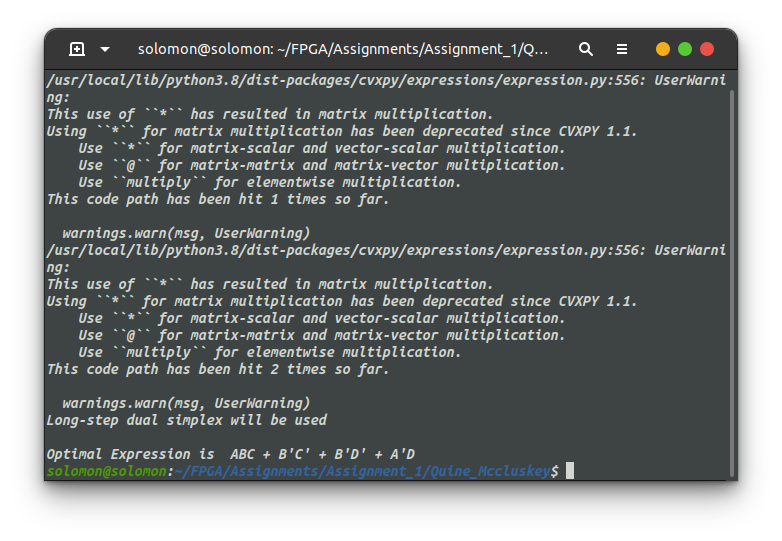
\includegraphics[scale=0.5]{./figs/opt.png}
\end{figure}

\textit{NOTE:- Here A, B, C, and D corresponds to P, Q, R, and S respectively.}
    
\subsection*{Boolean expression verification}
A \href{https://github.com/TUdayKiranReddy/FPGA_Lab/tree/main/Assignments/Assignment_1/codes/verification_testbench.c}{testbench} was created to verify the correctness of the obtained boolean expression.


\end{document}